\section{Implementation}
\label{sec:implementation}

\begin{figure}[tp]
\centering
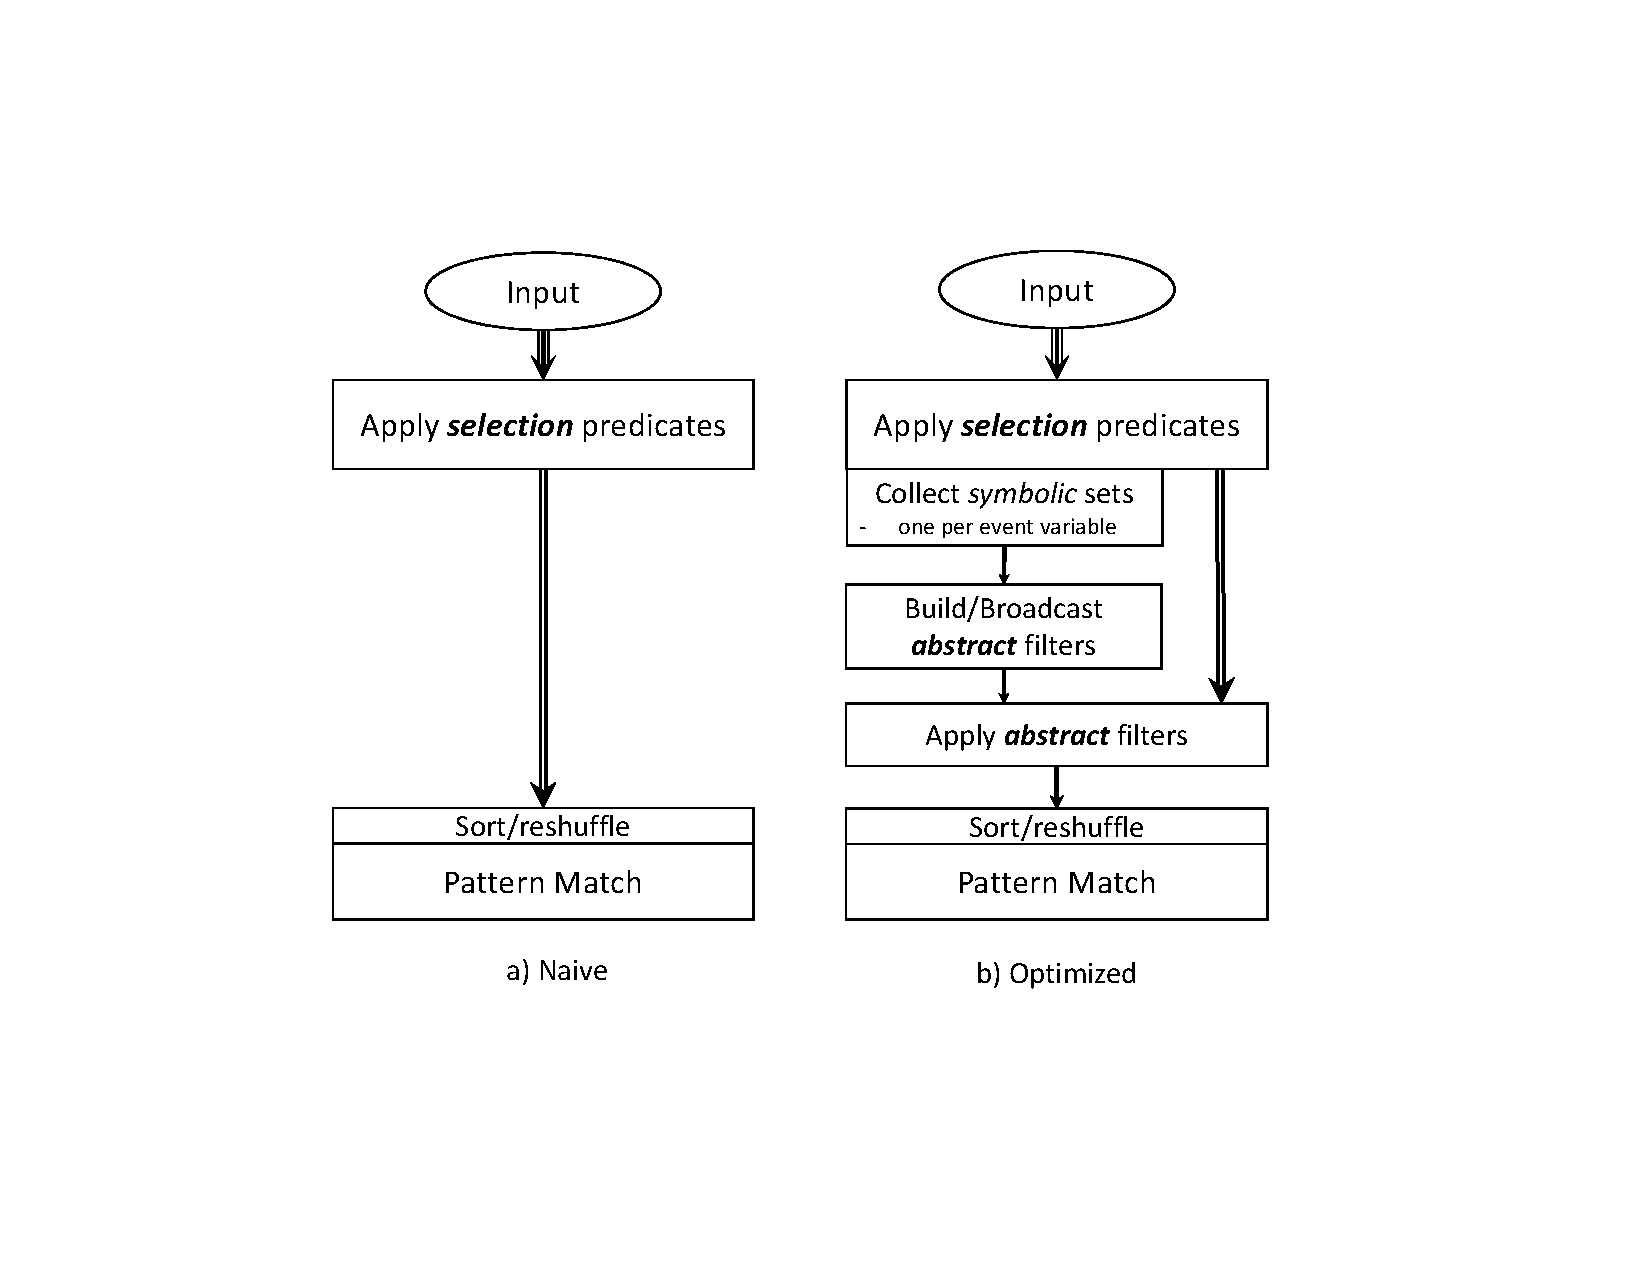
\includegraphics[clip, trim=5.6cm 4.5cm 6.3cm 4.2cm, 
width=0.45\textwidth]{graphs/query_plan.pdf}
\caption{Naive (i) and optimized (ii) execution plans for performing pattern 
matching on a map-reduce platform.}
\label{fig:query_plan}
\end{figure}


In the following we detail how we implemented our solution for speeding up 
large scale event series pattern matching on top of the 
Cosmos/Scope~\cite{Chaiken:2008} map-reduce framework.
We recall that the standard way of performing event-series pattern matching in 
such frameworks is to first remove all the events that do not match any of the 
selection predicates specified by the pattern, and then to sort on 
time/reshuffle the remaining events and finally process them using a pattern 
matching engine (see figure~\ref{fig:query_plan}(i)).

Our solution significantly extends the amount of data that gets filtered out 
during the preprocessing stage by constructing an {\em abstract} filter which 
also enforces the join predicates occurring in a pattern (as opposed to just 
the selection predicates).
The execution plan that we propose introduces 3 intermediary steps as is 
outlined in figure~\ref{fig:query_plan}(ii).
The first one collects in a parallel fashion a symbolic set for each event 
variable of the pattern (step 2a), followed by the union of these sets across 
all partitions of the input, and the results are then used to build the 
abstract filter by enforcing the join predicates between event variables (step 
2b). 
We then broadcast the abstract filter back to the preprocessing nodes and have 
them apply it over the output of the initial selection-predicate based filter 
(step 2c). 
Finally, the remaining events are sorted/reshuffled, just like in the standard 
approach and processed by the pattern matching engine. 


In implementing the execution plan in figure~\ref{fig:query_plan}(ii),
we make use as much as possible of the relational constructs and annotations 
provided by the Scope query language in order to maximize the potential for 
optimizations at the level of the entire data processing pipeline (for eg., we 
use native Scope to extract the event fields used in constructing the symbolic 
sets as well as to apply the filters that we build).
For operating with the set abstractions themselves we use the rich 
extensibility features of Scope, all the while providing hints to its query 
optimizer.

Even though the {\em abstract} filters have the potential to dramatically 
reduce the amount of data that gets sorted\allowbreak /\allowbreak 
reshuffled\allowbreak /\allowbreak pattern matched, 
constructing them introduces overheads both in terms of processing costs and 
latency.
In terms of processing costs we note that, while the construction of the 
symbolic sets can be done in the same pass as the selection-predicate based 
filtering, for applying the abstract filters we need a second pass over the 
data.
Nonetheless, since applying a filter is linear in the size of the input, this 
extra pass ends up being much cheaper than sorting on time the same input, and 
if the reduction ratio of the filter is considerable then applying it results 
in a net win. 
   
In terms of latency, our approach also introduces an extra reduction phase as 
required for aggregating the symbolic sets computed on each partition to a 
particular node where we can propagate the constraints specified by join 
predicates in order to obtain the abstract filters.
This is also followed by a broadcast phase that delivers the abstract filters 
back to the nodes processing the input stream.
In order to minimize the penalty in latency incurred by these two steps we 
limit the size of the abstract filters to the order of megabytes and we exploit 
the algebraic properties of the operators of the set abstractions that we use 
in order to optimize the aggregation (i.e.\ we make use of a {\em recursive} 
user defined aggregates).





  
  
  
  